% This file provides an example Beamer presentation using the RWTH theme
% showcasing some of the more common options, similar to the Powerpoint version
% 12.11.2014: Revision 1 (Harold Bruintjes, Tim Lange)

% For RWTH, beamer should be loaded with class option t (top)
\documentclass[t]{beamer}
%\documentclass[t,handout]{beamer}

% Use fontspec to get Arial font
% Requires use of XeLaTeX
%\usepackage{fontspec}
%\setmainfont{Arial}
%\setsansfont{Arial}
\usepackage[scaled=.90]{helvet}
\usepackage{subcaption}
%\usepackage{helvet}
% Also force Arial for math for a more consistent look
%\usepackage{unicode-math}
%\setmathfont{Arial}

% German style date formatting (footer)
%\usepackage[ddmmyyyy]{datetime}
%\renewcommand{\dateseparator}{.}

% Format the captions used for figures etc.
\usepackage[compatibility=false]{caption}
\captionsetup{singlelinecheck=off,justification=raggedleft,labelformat=empty,labelsep=none}

% PGFPlots is used for drawing some of the charts
%\usepackage{pgfplots}
%\pgfplotsset{compat=newest}
%\input{plot_commands.tex}

\usepackage[english]{babel}
\usepackage{tikz}
\usetikzlibrary{arrows.meta, positioning}

% Load the actual RWTH theme. Suggested is to load the full theme,
% as it requires some specific dimensions
\usetheme{rwth}

\setbeamercolor{math text}{fg=rwth}
\setbeamertemplate{theorems}[numbered]
\newtheorem{algorithm}[theorem]{Algorithm}

% Setup presentation information
\title{Large Language Models and Data Streams}
\subtitle{
  Seminar \textsl{Data Stream Management and Analysis}\\[1ex]
  \insertdate\\[1ex]
  \insertauthor
}
\date{\today}
\author{Silyu Li}
\institute{RWTH Aachen University}

% Set the logo to the file `logo`
% It will be scaled automatically
%\logo{
\includegraphics[scale=0.6]{rwth_i5_en_rgb.pdf}}
\logo{
\includegraphics[scale=0.5]{logo_new.png}}

% Uncomment this if you want a TOC at every section start
%\AtBeginSection[]{
%  \begin{frame}<beamer>{Outline}
%    \tableofcontents[currentsection]
%  \end{frame}
%}
%\AtBeginSubsection[]{
%  \begin{frame}<beamer>{Outline}
%    \tableofcontents[currentsection,currentsubsection]
%  \end{frame}
%}

% Use this to control some aspects of the footer
%\setbeamertemplate{footertextextra}{Extra text in the footer\enskip|\enskip{}Extra text in the footer}
\setbeamertemplate{footertext}{%
  \insertshorttitle\\[1ex]\insertauthor}

% Title page
\setbeamercolor{title page bar}{fg=white}
\setbeamertemplate{title page}[rwth][title_small]{}



\begin{document}
\begin{frame}[plain]
  \titlepage
\end{frame}

%\begin{frame}{Overview}
%  \tableofcontents
%\end{frame}

\section{Introduction}
\begin{frame}{Background}
  \begin{columns}
    \begin{column}{0.4\textwidth}
        \begin{figure}
            \centering
            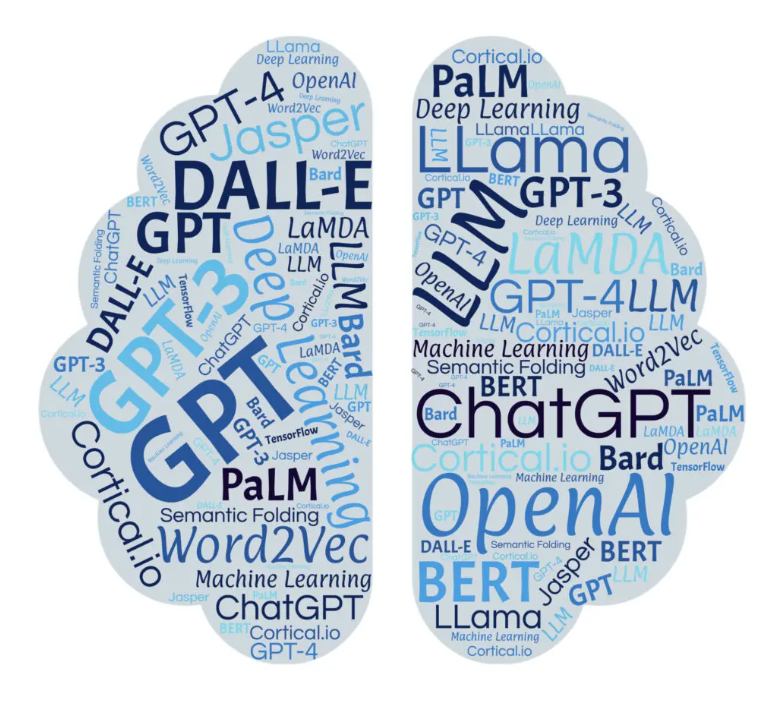
\includegraphics[width=\textwidth]{llm1.png}
            \caption{Relevant concepts of AI models and technologies\footnote{Source: \url{https://www.cortical.io/blog/chatgpt-and-large-language-models-the-holy-grail-of-enterprise-ai/}}}
            \label{fig:llm1}
        \end{figure}
    \end{column}
    \begin{column}{0.5\textwidth}
        \begin{itemize}
            \item LLM and AI have become very prominent topics in recent years.
        \end{itemize}
    \end{column}
\end{columns}
\end{frame}

\begin{frame}{Background}
\begin{figure}
  \centering
  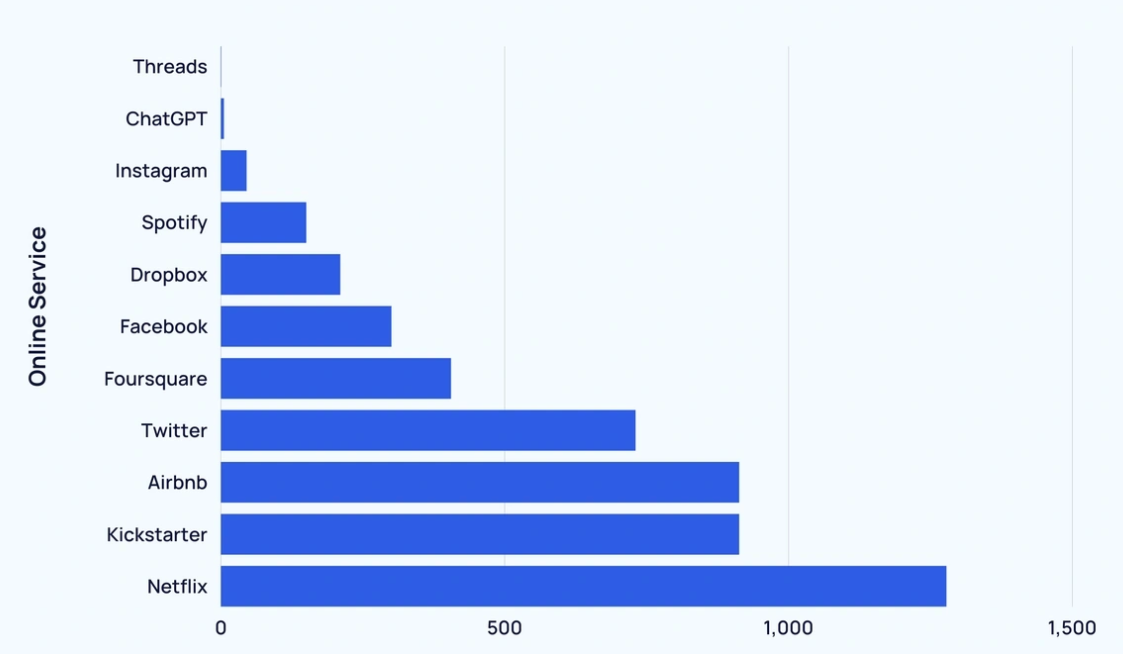
\includegraphics[width=0.7\textwidth]{1M users.png}
  \caption{Time needed for different Apps to have 1 million users\footnote{Source: \url{https://explodingtopics.com/blog/chatgpt-users}}}
\end{figure}
\end{frame}

\begin{frame}{Background}
  \begin{columns}
    \begin{column}{0.4\textwidth}
        \begin{figure}
            \centering
            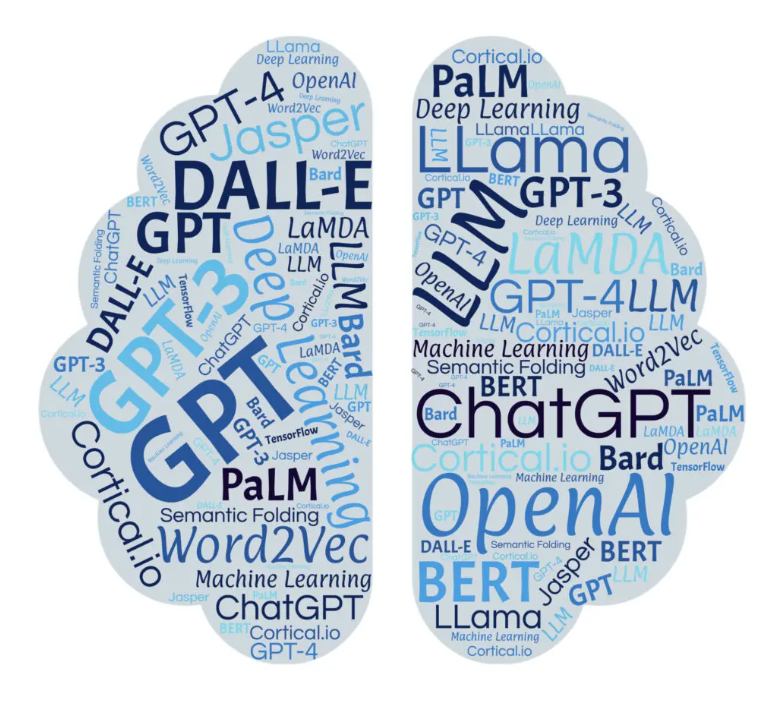
\includegraphics[width=\textwidth]{llm1.png}
            \caption{Relevant concepts of AI models and technologies\footnote{Source: \url{https://www.cortical.io/blog/chatgpt-and-large-language-models-the-holy-grail-of-enterprise-ai/}}}
            \label{fig:llm1}
        \end{figure}
    \end{column}
    \begin{column}{0.5\textwidth}
        \begin{itemize}
            \item LLM and AI have become very prominent topics in recent years.
            \newline
            \item Wide usage and significant competence in QA, content generation, translation, text classification and other tasks \cite{Liu23}.
        \end{itemize}
    \end{column}
\end{columns}
\end{frame}


\begin{frame}{Background}
  \begin{columns}
    \begin{column}{0.4\textwidth}
        \begin{figure}
            \centering
            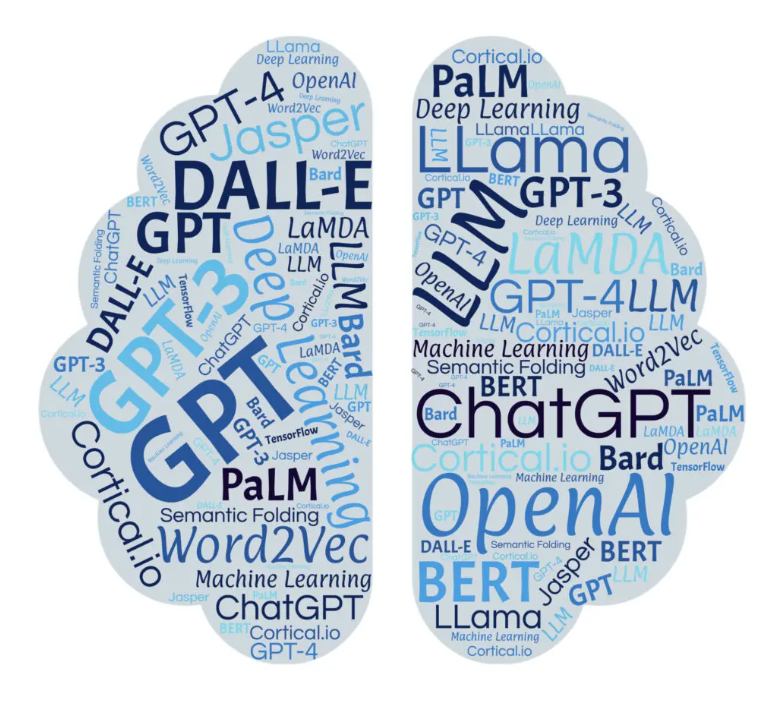
\includegraphics[width=\textwidth]{llm1.png}
            \caption{Relevant concepts of AI models and technologies\footnote{Source: \url{https://www.cortical.io/blog/chatgpt-and-large-language-models-the-holy-grail-of-enterprise-ai/}}}
            \label{fig:llm1}
        \end{figure}
    \end{column}
    \begin{column}{0.5\textwidth}
        \begin{itemize}
            \item LLM and AI have become very prominent topics in recent years.
            \newline
            \item Wide usage and significant competence in QA, content generation, translation, text classification and other tasks \cite{Liu23}.
            %\item QA, content generation, translation, text classification and other tasks \cite{Liu23}.
            \newline
            \item Most models are "static" \cite{Gupta23}.
        \end{itemize}
    \end{column}
\end{columns}
\end{frame}

\begin{frame}{Content}
  \vspace{1cm}
  \begin{itemize}
    \item Evolution of language models and the techniques behind them
    \newline
    \item Training process of several LLMs
    %\newline
    %\item Definition and application of data streams
    \newline
    \item Need, benefits, challenges and use cases of combining LLM with data streams
  \end{itemize}
\end{frame}
%------------------------------------------------------------------------------------------------------------
\begin{frame}{Large Language Models}
  \vspace{3cm}
  \centering
  \begin{tikzpicture}[
    %scale=2,
    timeline/.style={
        thick,
        -{Stealth[scale=1.5]},
        line cap=round,
    },
    event/.style={
        circle,
        draw,
        minimum size=12mm,
        fill=blue!20,
        inner sep=0pt,
        font=\footnotesize,
    },
    label/.style={
        font=\Large,
        anchor=south,
        text depth=0pt,
    }
]
    % Timeline
    \draw[timeline] (0,0) -- (3,0);
    
    % Events
    \node[event, label=below:{2000}] (event1) at (2,0) {1};
    
    % Event labels
    \node[label, above=of event1] {Simple Models};

\end{tikzpicture}
\vspace{1cm}
\begin{itemize}
  \item N-Gram \cite{Cavnar94}
  %\item Example: [("I", "read"), ("read", "a"), ("a", "book")]
  %\item .
  \item Calculate the next word's probability based on the N-1 previous sub-words.
  \item Poor performance on large documents and large N.
\end{itemize}
\end{frame}

\begin{frame}{N-Gram}
\vspace{1cm}
Example: Tri-Gram \\
\vspace{1cm}
Based on a text corpus, predict the next word of "I read"\\
\vspace{1cm}
$P("I","read","x") = Count("I","read","x")/Count("I","read")$
\end{frame}

\begin{frame}{Large Language Models}
  \vspace{3cm}
  \centering
  \begin{tikzpicture}[
    timeline/.style={
        thick,
        -{Stealth[scale=1.5]},
        line cap=round,
    },
    event/.style={
        circle,
        draw,
        minimum size=12mm,
        fill=blue!20,
        inner sep=0pt,
        font=\footnotesize,
    },
    label/.style={
        font=\Large,
        anchor=south,
        text depth=0pt,
    }
]
    % Timeline
    \draw[timeline] (0,0) -- (8,0);
    
    % Events
    \node[event, label=below:{2000}] (event1) at (1,0) {1};
    \node[event, label=below:{2005}] (event2) at (7,0) {2};
    %\node[event, label=below:{2010}] (event3) at (10,0) {3};
    %\node[event, label=below:{2015}] (event4) at (14,0) {4};
    %\node[event, label=below:{2020}] (event5) at (18,0) {5};
    
    % Event labels
    \node[label, above=of event1] {Simple Models};
    \node[label, above=of event2] {Shallow Neural Networks};
    %\node[label, above=of event3] {Neural Networks};
    %\node[label, above=of event4] {LSTM};
    %\node[label, above=of event5] {Transformers};
\end{tikzpicture}
\vspace{1cm}
\begin{itemize}
  \item Word2Vec \cite{Mikolov13}
  \item Map words into vector space.
  \item Similar words have a closer distance.
  \item Can capture contextual information.
  \item Better performance on large documents.
\end{itemize}
\end{frame}

\begin{frame}{Word2Vec}
  \vspace{1cm}
  Example \\
  \vspace{1cm}
  "I read a" $\Rightarrow$ $V_{I} + V_{read} + V_a$ \\
  \vspace{1cm}
  Compare similarity between $V_I + V_{read} + V_a$ and $V_I + V_{read} + V_a + V_x$
\end{frame}

\begin{frame}{Large Language Models}
  \vspace{3cm}
  \centering
  \begin{tikzpicture}[
    timeline/.style={
        thick,
        -{Stealth[scale=1.5]},
        line cap=round,
    },
    event/.style={
        circle,
        draw,
        minimum size=12mm,
        fill=blue!20,
        inner sep=0pt,
        font=\footnotesize,
    },
    label/.style={
        font=\Large,
        anchor=south,
        text depth=0pt,
    }
]
    % Timeline
    \draw[timeline] (0,0) -- (12,0);
    
    % Events
    \node[event, label=below:{2000}] (event1) at (1,0) {1};
    \node[event, label=below:{2005}] (event2) at (6,0) {2};
    \node[event, label=below:{2010}] (event3) at (10,0) {3};
    %\node[event, label=below:{2015}] (event4) at (14,0) {4};
    %\node[event, label=below:{2020}] (event5) at (18,0) {5};
    
    % Event labels
    \node[label, above=of event1] {Simple Models};
    \node[label, above=of event2] {Shallow Neural Networks};
    \node[label, above=of event3] {RNN};
    %\node[label, above=of event4] {LSTM};
    %\node[label, above=of event5] {Transformers};
\end{tikzpicture}
\vspace{1cm}
\begin{itemize}
  \item Seq2Seq \cite{Sutskever14}
  \item Specially designed architecture to obtain long-term dependencies.
  %\item Encodes input into vectors with fixed dimensionality and decodes them.
  \item Much better performance on large documents, can work with different input lengths.
  \item But still problematic on very large documents.
\end{itemize}
\end{frame}

\begin{frame}{Seq2Seq}
  \vspace{1cm}
  Example \\
  \vspace{1cm}
  "I read a book \dots" $\Rightarrow$ $\{"I"\}$ $\Rightarrow$ $\{"read"\}$ $\Rightarrow$ $\{"a"\}$ $\Rightarrow$ $\{"book"\}$
  $\Rightarrow$ \dots \\
\end{frame}

\begin{frame}{Large Language Models}
  \vspace{3cm}
  \centering
  \begin{tikzpicture}[
    timeline/.style={
        thick,
        -{Stealth[scale=1.5]},
        line cap=round,
    },
    event/.style={
        circle,
        draw,
        minimum size=12mm,
        fill=blue!20,
        inner sep=0pt,
        font=\footnotesize,
    },
    label/.style={
        font=\Large,
        anchor=south,
        text depth=0pt,
    }
]
    % Timeline
    \draw[timeline] (0,0) -- (16,0);
    
    % Events
    \node[event, label=below:{2000}] (event1) at (1,0) {1};
    \node[event, label=below:{2005}] (event2) at (6,0) {2};
    \node[event, label=below:{2010}] (event3) at (10,0) {3};
    %\node[event, label=below:{2015}] (event4) at (14,0) {4};
    \node[event, label=below:{2020}] (event4) at (14,0) {5};
    
    % Event labels
    \node[label, above=of event1] {Simple Models};
    \node[label, above=of event2] {Shallow Neural Networks};
    \node[label, above=of event3] {RNN};
    %\node[label, above=of event4] {LSTM};
    \node[label, above=of event4] {Transformers};
\end{tikzpicture}
\vspace{1cm}
\begin{itemize}
  \item Transformer \cite{Vaswani17}
  %\item Works with the self-attention mechanism.
  \item Can process the entire input sentence simultaneously.
  \item Very good performance on large documents, more efficient and powerful.
\end{itemize}
\end{frame}

\begin{frame}{Transformer}
  \vspace{1cm}
  Example \\
  \vspace{1cm}
  "I read a book \dots" $\Rightarrow$ $\{"I_1" "read_2" "a_3" "book_4" \dots\}$
\end{frame}

\begin{frame}{Large Language Models}
  \vspace{3cm}
  \centering
  \begin{tikzpicture}[
    timeline/.style={
        thick,
        -{Stealth[scale=1.5]},
        line cap=round,
    },
    event/.style={
        circle,
        draw,
        minimum size=12mm,
        fill=blue!20,
        inner sep=0pt,
        font=\footnotesize,
    },
    label/.style={
        font=\Large,
        anchor=south,
        text depth=0pt,
    }
]
    % Timeline
    \draw[timeline] (0,0) -- (20,0);
    
    % Events
    \node[event, label=below:{2000}] (event1) at (1,0) {1};
    \node[event, label=below:{2005}] (event2) at (6,0) {2};
    \node[event, label=below:{2010}] (event3) at (10,0) {3};
    \node[event, label=below:{2015}] (event4) at (14,0) {4};
    \node[event, label=below:{2020}] (event5) at (18,0) {5};
    
    % Event labels
    \node[label, above=of event1] {Simple Models};
    \node[label, above=of event2] {Shallow Neural Networks};
    \node[label, above=of event3] {RNN};
    \node[label, above=of event4] {Transformers};
    \node[label, above=of event5] {Recent Models};
\end{tikzpicture}
\vspace{1cm}
\begin{itemize}
  \item BERT, ChatGPT, LLaMA\dots
  \item Based on the transformer architecture.
  \item Trained on massive datasets and fine-tuned with downstream tasks.
  %\item Very good performance on large documents, more efficient and powerful.
\end{itemize}
\end{frame}

\section{Training Process of LLMs}
\begin{frame}{Tokenization}
  \begin{itemize}
    \item Purpose: Segmenting input text into tokens, which are elements from the vocabulary that the model knows.
    \newline
    \item BERT: "I read a book" $\Rightarrow$ ["I", "re", "\#\#ad", "a", "book"] \cite{Wu16}
    \newline
    \item GPT2, LLaMA: "I read a book" $\Rightarrow$ [\dots, "re","ad",\dots] $\Rightarrow$ [\dots, "read",\dots] \cite{Sennrich15}
    %\item Sentence Piece (LLaMA)
  \end{itemize}
\end{frame}

\begin{frame}{Pre-training}
Given an unlabeled corpus of tokens $U=\{u_1,...,u_n\}$ as a training dataset, the core idea of the pre-training phase is to 
predict the next token $u_i$ for a sequence $\{u_{i-k},...,u_{i-1}\}$, specifically by maximizing the likelihood: 
\begin{equation}
  L_1(U) = \sum_{i}\log{P(u_i|u_{i-k},...,u_{i-1}; \Theta)} \cite{Radford18}
\end{equation}
$k$ refers to the context window size and $\Theta$ is the parameter of the neural network with which the conditional probability $P$ is modeled.
\end{frame}


\begin{frame}{Example: BERT \cite{Devlin18}}
  \vspace{1cm}
  \begin{itemize}
    \item Next Sentence Prediction (Pre-training phase)
    \begin{itemize}
      \item BERT is trained to predict if the second sentence B (of longer sentence A, B) is real, with B being replaced by a random sentence half the time.
      \item "I read a book", "it is amazing" or "I read a book", "The weather is bad".
    \end{itemize}
  \end{itemize}
\end{frame}

\begin{frame}{Fine-tuning}
  Given a labeled dataset $C$,
  where each instance of $C$ has a sequence of tokens \{$c^1,...,c^m$\} and a label $y$, the goal of the fine-tuning phase is to maximize the following likelihood:
  \begin{equation}
    L_2(U) = \sum_{(c,y)}\log{P(y|c^1,...,c^m)} \cite{Radford18}
  \end{equation}
\end{frame}

\begin{frame}{Example: BERT \cite{Devlin18}}
  \vspace{1cm}
  \begin{itemize}
    \item Next Sentence Prediction (Pre-training phase)
    \begin{itemize}
      \item BERT is trained to predict if the second sentence B (of longer sentence A, B) is real, with B being replaced by a random sentence half the time.
      \item "I read a book", "it is amazing" or "I read a book", "The weather is bad".
    \end{itemize}
    \vspace{1cm}
    \item Question Answering (Fine-tuning phase)
    \begin{itemize}
      \item Bert uses the Stanford Question Answering Dataset that contains 100k question/answer pairs.
    \end{itemize}
  \end{itemize}
\end{frame}

\begin{frame}{A Comparison of Different Models}
  %\vspace{1cm}
  \begin{table}[H]
    \centering
    \small
    \begin{tabular}{| p{4cm} | p{2cm} | p{2cm} | p{2cm} | p{2cm} |}
    \hline
    \textbf{Model Name} & BERT & GPT-2 & LLaMA & GPT-3,5/ 4 \\
    \hline
    \textbf{Developer} & GoogleAI & OpenAI & MetaAI & OpenAI \\
    \hline
    \textbf{Release Date} & 2018 & 2019 & 2023 & 2022/2023 \\
    \hline
    \textbf{Nr. of Parameters} & 110 M/ 340 M & 1,5 B & 7-65 B & 175 B/1,7 T \\
    \hline
    \textbf{Training Data} & Wikipedia(en) \& BookCorpus\footnote{\url{https://en.wikipedia.org/wiki/BookCorpus}} & WebText & Various open-source datasets & WebText \\
    \hline
    \textbf{Open-sourced} & Yes & No & Yes & No \\
    \hline
    \textbf{Major Applications} & QA & Text generation \& Translation & Text generation \& QA \& Translation & Content generation \& QA \& Translation \\
    \hline
    \end{tabular}
    \caption{Comparison of Large Language Models}
    \label{table:comparison}
  \end{table}
\end{frame}

\begin{frame}{A Comparison of Different Models}
  %\vspace{1cm}
  \begin{table}[H]
    \centering
    \small
    \begin{tabular}{| p{4cm} | p{2cm} | p{2cm} | p{2cm} | p{2cm} |}
    \hline
    \textbf{Model Name} & BERT & GPT-2 & LLaMA & GPT-3,5/ 4 \\
    \hline
    \textbf{Developer} & GoogleAI & OpenAI & MetaAI & OpenAI \\
    \hline
    \textbf{Release Date} & 2018 & 2019 & 2023 & 2022/2023 \\
    \hline
    \textbf{Nr. of Parameters} & 110 M/ 340 M & 1,5 B & 7-65 B & 175 B/1,7 T \\
    \hline
    \textbf{Training Data} & Wikipedia(en) \& BookCorpus\footnote{\url{https://en.wikipedia.org/wiki/BookCorpus}} & WebText & Various open-source datasets & WebText \\
    \hline
    \textbf{Open-sourced} & Yes & No & Yes & No \\
    \hline
    \textbf{Major Applications} & QA & Text generation \& Translation & Text generation \& QA \& Translation & Content generation \& QA \& Translation \\
    \hline
    \end{tabular}
    \caption{Comparison of Large Language Models}
    \label{table:comparison}
  \end{table}
  The performance of a model increases exponentially when either one of the following factors are scaled up: 
  the number of model parameters, the size of training datasets and the available computational resource \cite{Kaplan20}.
\end{frame}

\section{LLM with Data Streams}
%\subsection{Continual Learning}
\begin{frame}{Data Stream}
  \vspace{1cm}
  \begin{definition}
    A data stream $S$ is an unbounded, potentially infinite multiset of data stream elements $(s,\tau)$, where $\tau \in \mathbb{T}$.
     $\mathbb{T}$ is a timestamp attribute with values from a monotonic, infinite time domain $\mathbb{T}$ with discrete time units. \cite{Geisler13}
  \end{definition}
\end{frame}

\begin{frame}{Limitations of Pre-trained LLMs}
  \vspace{1cm}
  \begin{itemize}
    \item Lack of knowledge beyond the scope of their training datasets.
    \newline
    \item The performance is likely to gradually degrade over time when finetuned on new tasks \cite{Shi24}.
    \newline
    \item Extremely computationally expensive to be re-trained.
    %\newline
    %\item Not able to process data streams as input.
  \end{itemize}
\end{frame}

\section{LLMs and Data Streams}
\begin{frame}{Application Fields: Traffic Data}
  \begin{figure}
    \centering
    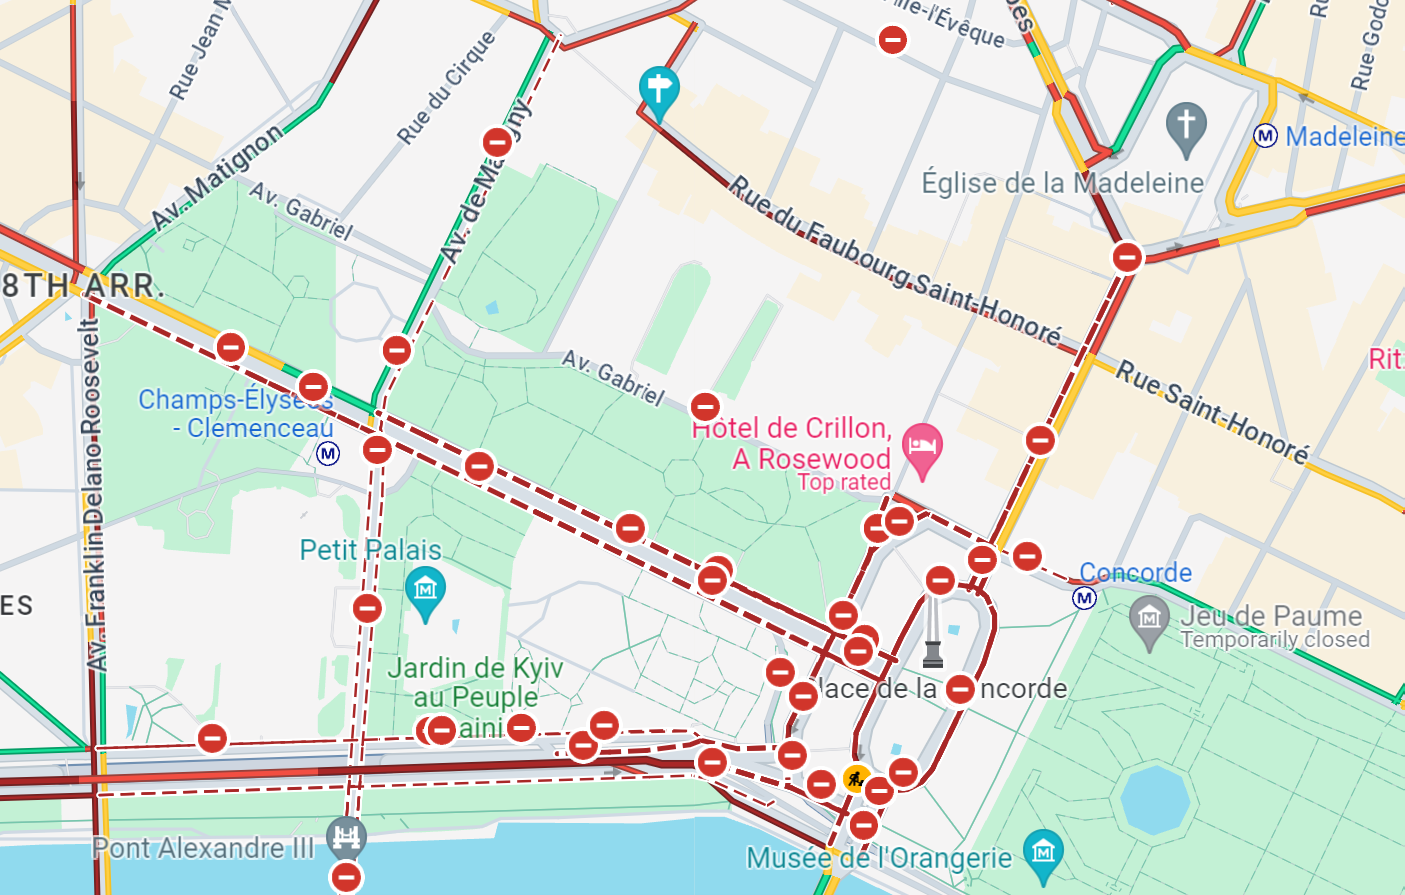
\includegraphics[width=0.6\textwidth]{paris_traffic.png}
    \caption{A screenshot of traffic in Paris using Google Maps\footnote{Source: \url{https://www.google.com/maps/}}}
    \label{fig:paris}
\end{figure}
\end{frame}

\begin{frame}{Application Fields: Social Media}
  \begin{figure}
    \centering
    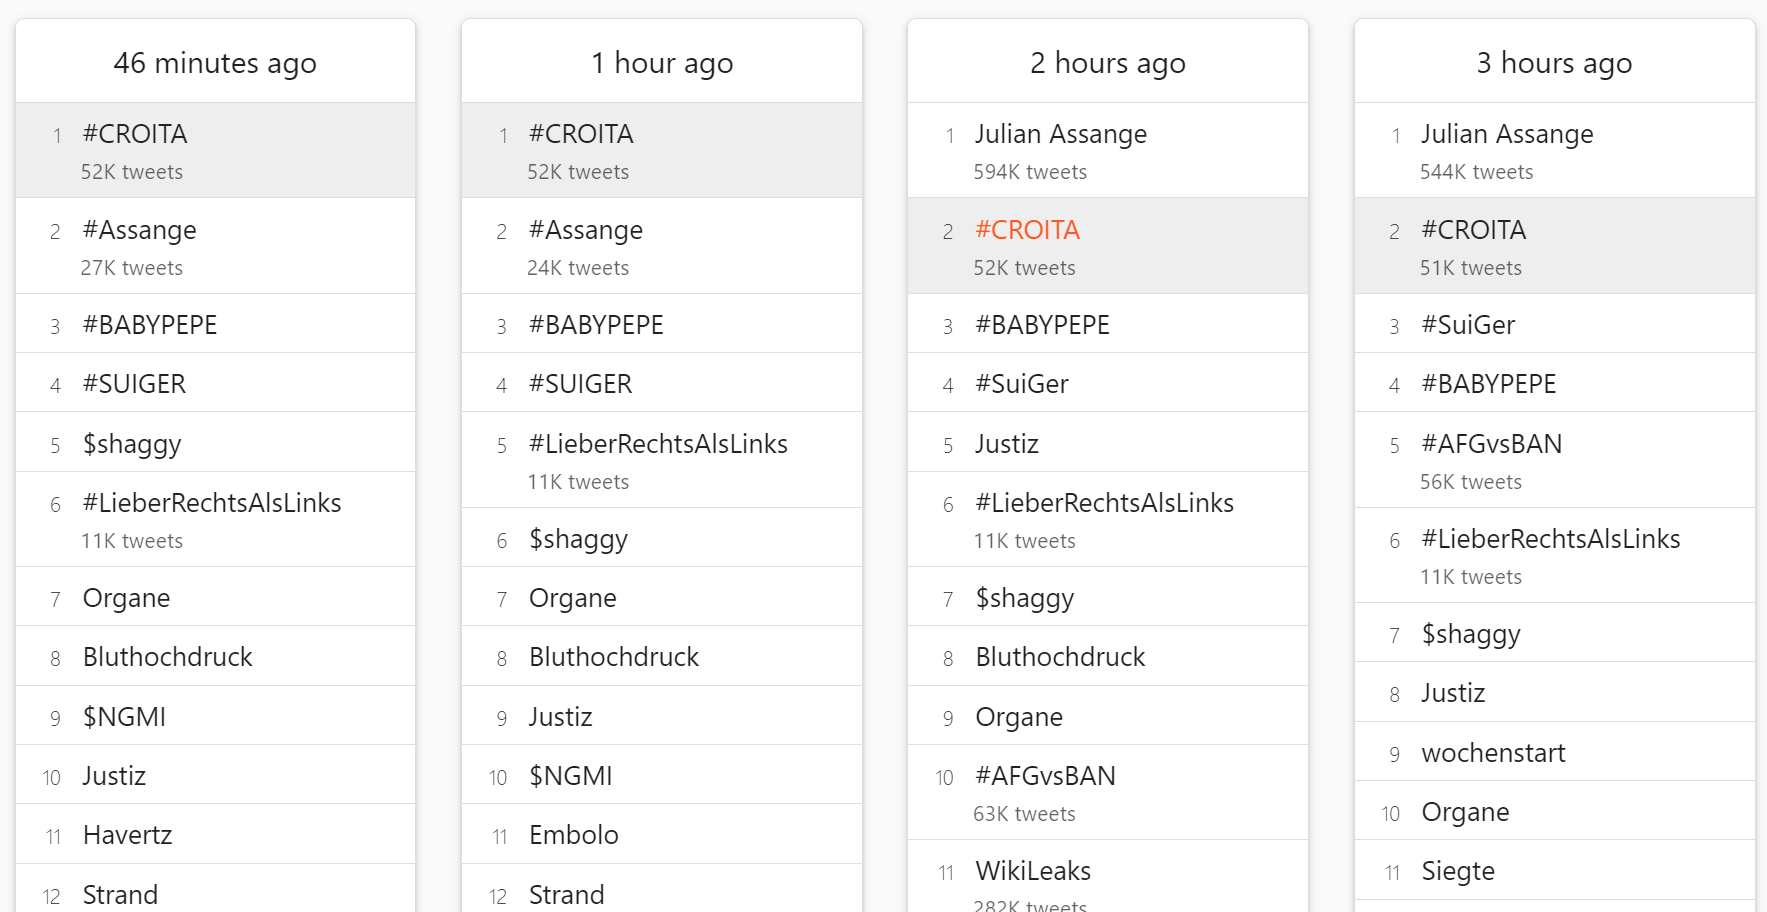
\includegraphics[width=0.7\textwidth]{trends.png}
    \caption{Current Twitter trending topics in Germany \footnote{Source: \url{https://trends24.in/germany/}}}
    \label{fig:trend}
\end{figure}
\end{frame}

\begin{frame}{Solution 1}
  \vspace{5cm}
  \centering
  Prompt Engineering 
\end{frame}

%\subsection{Prompt Engineering}
\begin{frame}{Prompt Engineering}
  \vspace{1cm}
  \begin{definition}{A prompt}
    is a set of instructions provided to an LLM that programs the LLM by customizing it and/or enhancing or refining its capabilities  
  \end{definition}
\end{frame}
\begin{frame}{Prompt Engineering}
  \vspace{1cm}
  \begin{definition}{A prompt}
    is a set of instructions provided to an LLM that programs the LLM by customizing it and/or enhancing or refining its capabilities. \cite{LiuPengfei23}   
  \end{definition}
  \vspace{1cm}
  \begin{definition}{Prompt Engineering}
    is the means by which LLMs are programmed via prompts. \cite{LiuPengfei23}  
  \end{definition}
\end{frame}

\begin{frame}{Prompt Engineering}
  \begin{figure}[htbp]
    \centering
    \begin{subfigure}[b]{0.42\textwidth}
        \centering
        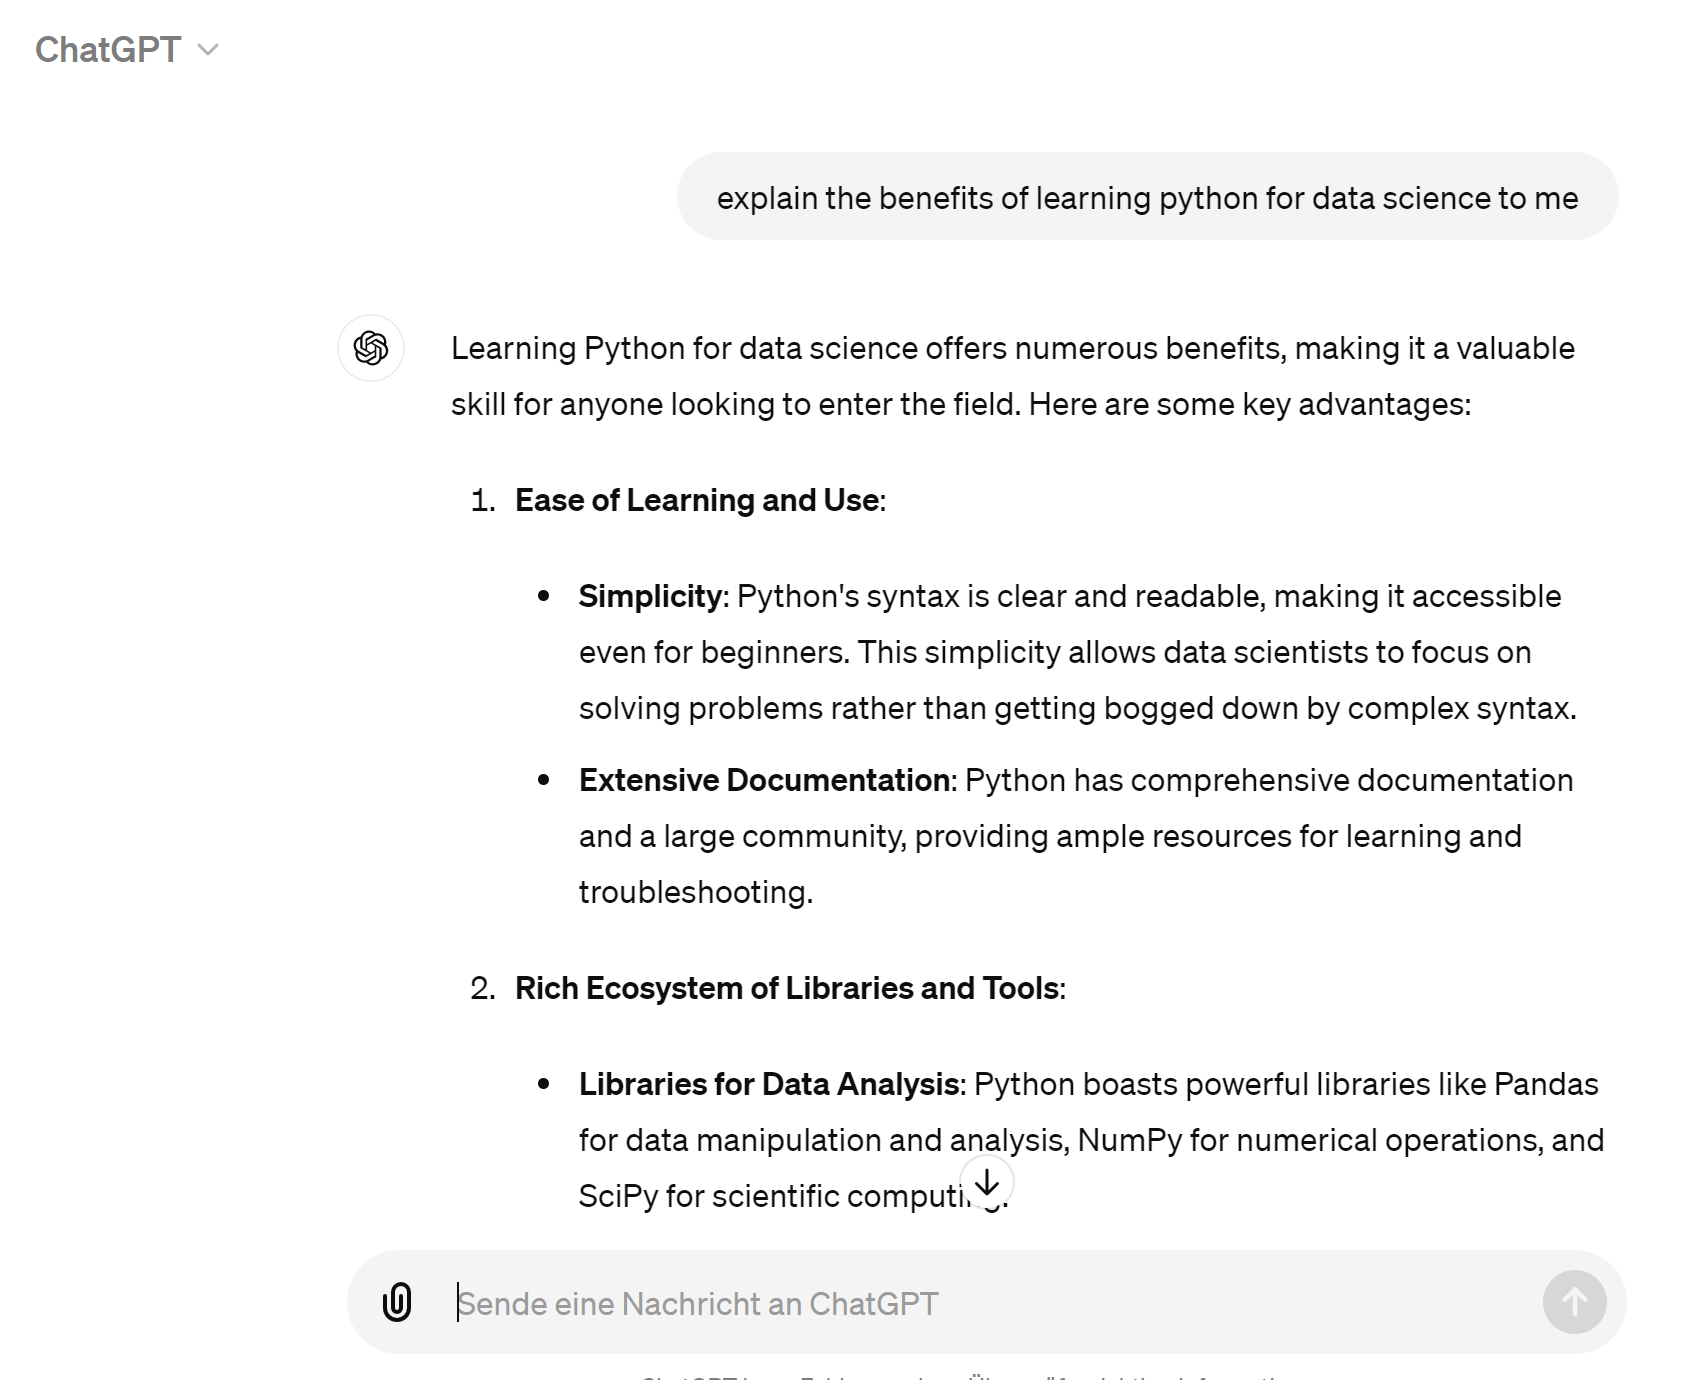
\includegraphics[width=\textwidth]{prompt_ds_1.PNG}
        \caption{Prompt 1}
        \label{fig:prompt1}
    \end{subfigure}
    \hfill
    \begin{subfigure}[b]{0.42\textwidth}
        \centering
        
\includegraphics[width=\textwidth]{prompt_ds_2.PNG}
        \caption{Prompt 2}
        \label{fig:prompt2}
    \end{subfigure}
    \caption{2 different prompts yield different output of ChatGPT}
    \label{fig:both_prompts}
  \end{figure}
\end{frame}

\begin{frame}{Use Case: LLMLight}
  \begin{figure}
    \centering
    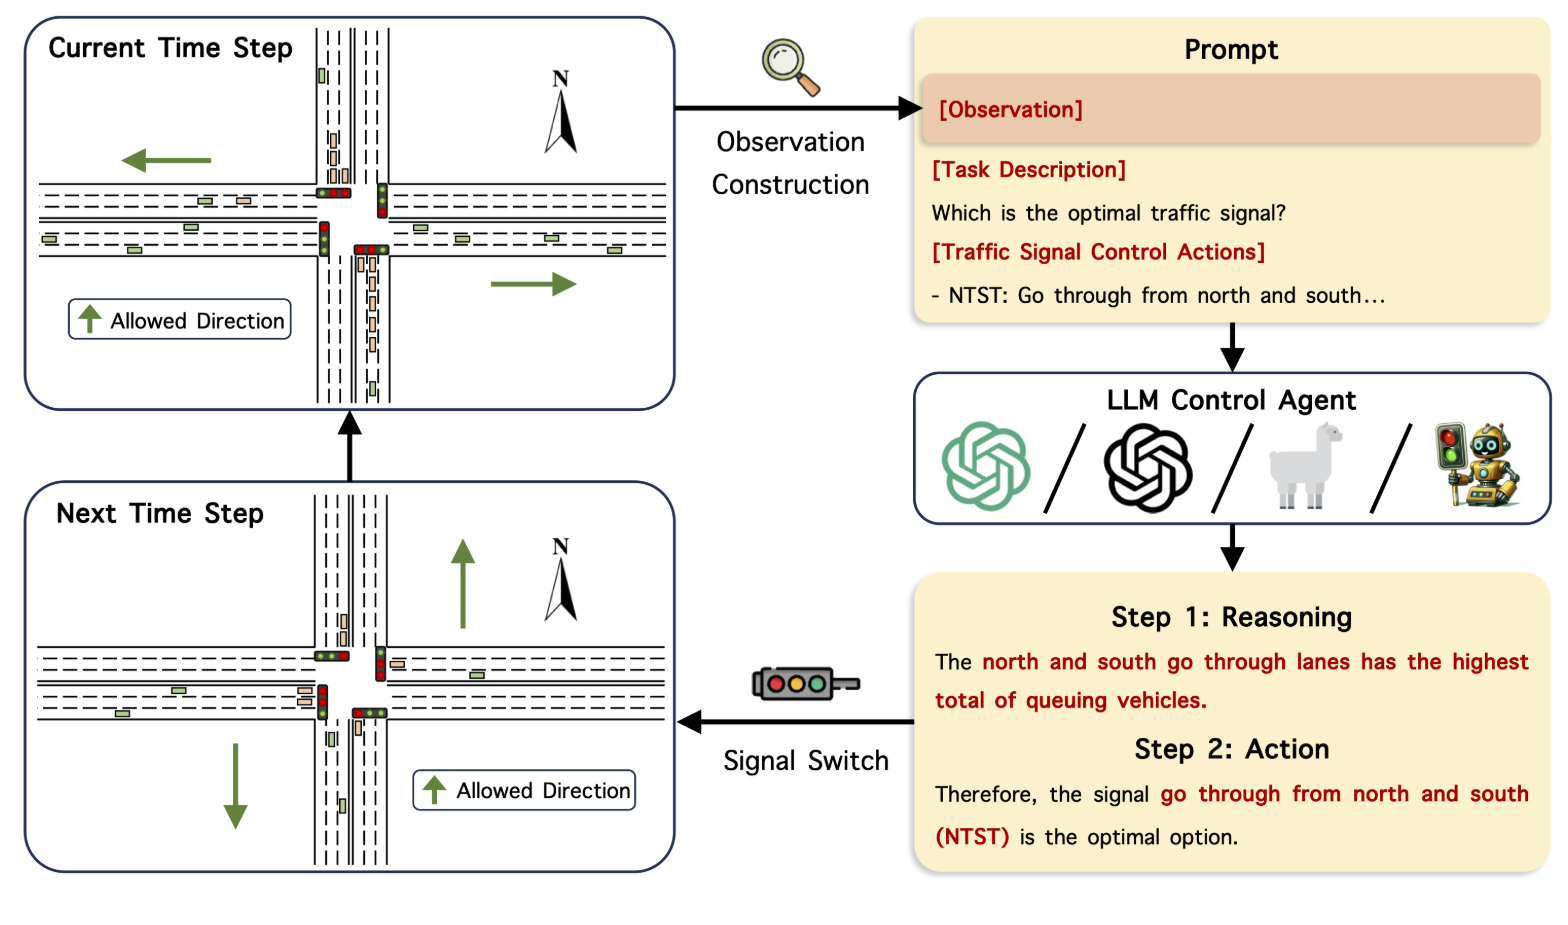
\includegraphics[width=0.7\textwidth]{LLMLight.PNG}
    \caption{The workflow of LLMLight \cite{Lai23}}
    \label{fig:llmlight}
\end{figure}
\end{frame}

\begin{frame}{Prompt Engineering}
  \vspace{1cm}
  \begin{itemize}
    \item Convert the real-time data into model-readable prompts and update the model’s knowledge via prompt engineering.
    %\item However, this method heavily relies on the quality of the prompt formulated by users.
  \end{itemize}
\end{frame}

\begin{frame}{Prompt Engineering}
  \vspace{1cm}
  \begin{itemize}
    \item Convert the real-time data into model-readable prompts and update the model’s knowledge via prompt engineering.
    \newline
    \item However, this method heavily relies on the quality of the prompt formulated by users.
  \end{itemize}
\end{frame}

\begin{frame}{Prompt Engineering}
  \vspace{1cm}
  \begin{itemize}
    \item Convert the real-time data into model-readable prompts and update the model’s knowledge via prompt engineering.
    \newline
    \item However, this method heavily relies on the quality of the prompt formulated by users.
    \newline
    \item A domain specific LLM is needed.
  \end{itemize}
\end{frame}

\begin{frame}{Solution 2}
  \vspace{5cm}
  \centering
  Continual Learning 
\end{frame}

\begin{frame}{Continual Learning}
  \vspace{1cm}
  \begin{Definition}
    continual learning refers to the process of accumulating knowledge on non-stationary data. In the context of large language models, continual learning is applied to enable LLMs
to learn from a continuous data stream over time. \cite{Biesi20}
  \end{Definition}
\end{frame}
\begin{frame}{Continual Learning}
  \vspace{1cm}
  \begin{Definition}
    continual learning refers to the process of accumulating knowledge on non-stationary data. In the context of large language models, continual learning is applied to enable LLMs
to learn from a continuous data stream over time. \cite{Biesi20}
  \end{Definition}
  \vspace{1cm}
  \begin{Definition}
    For a data stream of tasks $\mathcal{T}= \{\mathcal{T}_1,\ldots,\mathcal{T}_n \}$, the goal is to
have the model learn sequentially based on the input stream, where it only has access to $\mathcal{T}_i$ at time $i$. \cite{Wu24}
  \end{Definition}
\end{frame}

\begin{frame}{Stages of Continual Learning\cite{Wu24}}
  \vspace{1cm}
  \begin{itemize}
    \item \textbf{Continual Pre-training (CPT)}: It refers to incrementally updating a large language model on input data over time without retraining it from scratch. 
    \newline
    \item \textbf{Continual Instruction Tuning (CIT)}: It refers to continuously refining the model's ability to follow the instruction. 
    \newline
    \item \textbf{Continual Alignment (CA)}: It refers to adjusting the model so it always produces output that satisfies certain standards and guidelines. 
  \end{itemize}
\end{frame}

\begin{frame}{Stages of Continual Learning}
  \vspace{1cm}
  \begin{figure}[htbp]
    \centering
    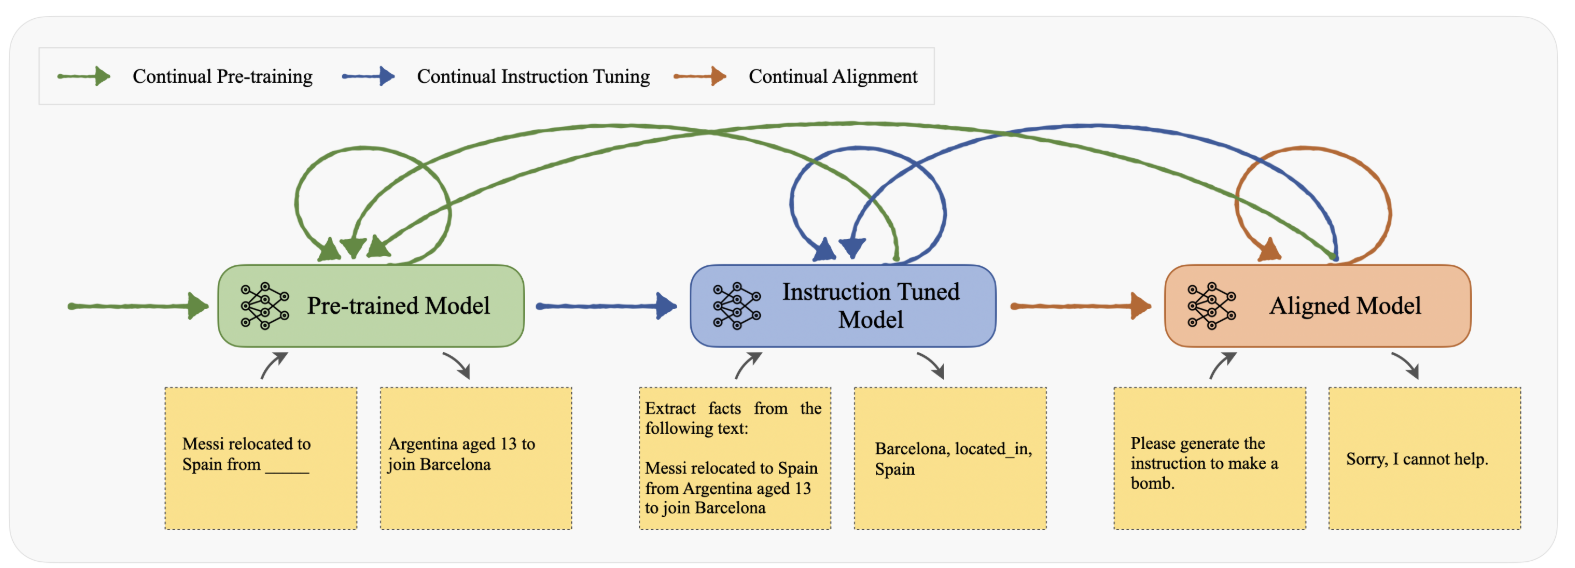
\includegraphics[width=0.95\textwidth]{CL stages.png}
    \caption{Stages of continual learning \cite{Wu24}}
    \label{fig:acl_stages}
  \end{figure}
\end{frame}

\begin{frame}{Continual Learning}
  \vspace{1cm}
  However, during continual learning on new input streams, models are likely to forget
  previously learned knowledge (Catastrophic Forgetting). \cite{Gupta23}
\end{frame}

\begin{frame}{Continual Learning}
  \vspace{1cm}
  However, during continual learning on new input streams, models are likely to forget
  previously learned knowledge (Catastrophic Forgetting). \cite{Gupta23}
  \vspace{1cm}
  \begin{itemize}
    \item Replay-based methods
    \item Regularization-based methods
    \item Architecture-based Methods
  \end{itemize}
\end{frame}

%\begin{frame}{Use Case: Swallow}
%  \vspace{1cm}
%  \begin{itemize}
%    \item Some large language models are trained on English datasets and their performance in other languages differs from their performance in English.
%    \newline
%    \item Develop a large language model Swallow that has strong performance in Japanese using continual learning methods based on LLaMA 2.
%    \newline
%    \item Swallow preserves the same architecture as LLaMA 2.
%    \newline
%    \item Apply the replay-based method by selecting 5\% of the training data from English datasets, 5\% from the English arXiv paper texts and the remaining 90\% from Japanese texts.
%    \newline
%    \item Evaluate the performance in various fields such as question answering (QA), reading com-
%    prehension (RC), automatic summarization (AS) and so on.
%  \end{itemize}
%\end{frame}

%\begin{frame}{Use Case: Swallow}
%  \begin{figure}[htbp]
%    \centering
%    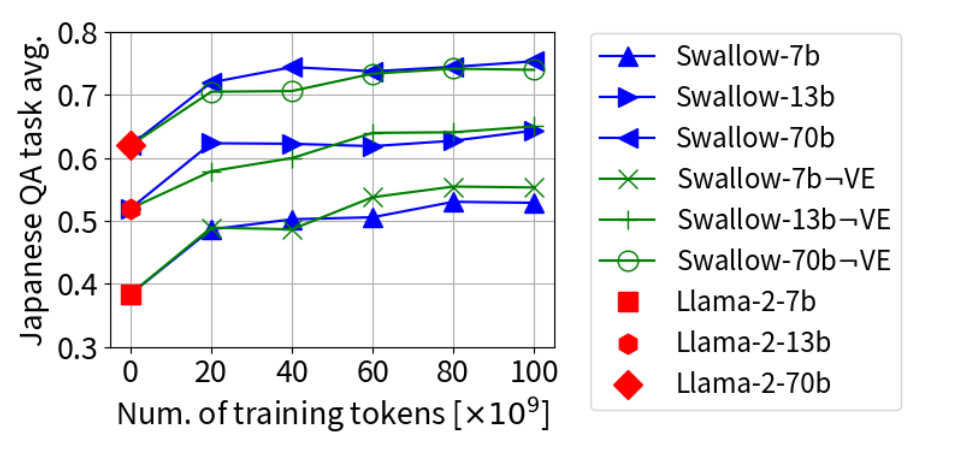
\includegraphics[width=0.9\textwidth]{swallow.png}
%    \caption{Performance curve of the Swallow model in question answering task \cite{Fujii24}}
%    \label{fig:progressive}
%  \end{figure}
%\end{frame}

\begin{frame}{Challenges of Continual Learning \cite{Gupta23}, \cite{Yang24}}
  \vspace{1cm}
  \begin{itemize}
    \item Catastrophic forgetting
    \newline
    \item Lack of real-world assumption
    \newline
    \item Multi-modal continual learning
    \newline
    \item Concept drift
  \end{itemize}
\end{frame}

\section{Conclusion}
\begin{frame}{}
  \vspace{1cm}
  \begin{itemize}
    \item Several models such as ChatGPT and GPT4 are not open-sourced, their exact training process and architecture details remain unknown.
    \newline
    \item Real-world applications of the two methods are still very limited.
    \newline
    \item In reality, data is often irregular and multi-modal, making
    it costly to transform into a usable format.
    \newline
    \item Implement more efficient algorithms to reduce the computational overhead of CA while mitigating catastrophic forgetting
    \newline
    \item Develop more effective prompt generation processes.
    \newline
    \item Explore more real-world applications.
  \end{itemize}
\end{frame}

\section{References}

\begin{frame}[allowframebreaks]
  \begin{thebibliography}{}
    \bibitem{Liu23}
    Liu, Yiheng, Tianle Han, Siyuan Ma, Jiayue Zhang, Yuanyuan Yang, Jiaming Tian, Hao He et al. "Summary of chatgpt-related research and perspective towards the future of large language models." Meta-Radiology (2023): 100017.
    \bibitem{Gupta23}
    Gupta, Kshitij, Benjamin Thérien, Adam Ibrahim, Mats L. Richter, Quentin Anthony, Eugene Belilovsky, Irina Rish, and Timothée Lesort. "Continual Pre-Training of Large Language Models: How to (re) warm your model?." arXiv preprint arXiv:2308.04014 (2023).  
    \bibitem{Cavnar94}
    Cavnar, William B., and John M. Trenkle. "N-gram-based Text Categorization." In Proceedings of SDAIR-94, 3rd Annual Symposium on Document Analysis and Information Retrieval, 161-175. Las Vegas, NV, 1994. Ann Arbor, MI: Environmental Research Institute of Michigan (ERIM).
    \bibitem{Mikolov13}
    Mikolov, Tomas, Ilya Sutskever, Kai Chen, Greg S. Corrado, and Jeff Dean. "Distributed representations of words and phrases and their compositionality." Advances in neural information processing systems 26 (2013).
    \bibitem{Sutskever14}
Sutskever, Ilya, Oriol Vinyals, and Quoc V. Le. "Sequence to sequence learning with neural networks." Advances in neural information processing systems 27 (2014).

\bibitem{Vaswani17}
Vaswani, Ashish, Noam Shazeer, Niki Parmar, Jakob Uszkoreit, Llion Jones, Aidan N. Gomez, Łukasz Kaiser, and Illia Polosukhin. "Attention is all you need." Advances in neural information processing systems 30 (2017).

\bibitem{Devlin18}
Devlin, Jacob, Ming-Wei Chang, Kenton Lee, and Kristina Toutanova. "Bert: Pre-training of deep bidirectional transformers for language understanding." arXiv preprint arXiv:1810.04805 (2018).

\bibitem{Wu16}
Wu, Yonghui, Mike Schuster, Zhifeng Chen, Quoc V. Le, Mohammad Norouzi, Wolfgang Macherey, Maxim Krikun et al. "Google's neural machine translation system: Bridging the gap between human and machine translation." arXiv preprint arXiv:1609.08144 (2016).
  
\bibitem{Sennrich15}
Sennrich, Rico, Barry Haddow, and Alexandra Birch. "Neural machine translation of rare words with subword units." arXiv preprint arXiv:1508.07909 (2015).

\bibitem{Radford18}
Radford, Alec, Karthik Narasimhan, Tim Salimans, and Ilya Sutskever. "Improving language understanding by generative pre-training." (2018).

\bibitem{Geisler13}
Geisler, Sandra. "Data stream management systems." In Dagstuhl Follow-Ups, vol. 5. Schloss Dagstuhl-Leibniz-Zentrum fuer Informatik, 2013.

\bibitem{Shi24}
Shi, Haizhou, Zihao Xu, Hengyi Wang, Weiyi Qin, Wenyuan Wang, Yibin Wang, and Hao Wang. "Continual Learning of Large Language Models: A Comprehensive Survey." arXiv preprint arXiv:2404.16789 (2024).

\bibitem{LiuPengfei23}
Liu, Pengfei, Weizhe Yuan, Jinlan Fu, Zhengbao Jiang, Hiroaki Hayashi, and Graham Neubig. "Pre-train, prompt, and predict: A systematic survey of prompting methods in natural language processing." ACM Computing Surveys 55, no. 9 (2023): 1-35.

\bibitem{Lai23}
Lai, Siqi, Zhao Xu, Weijia Zhang, Hao Liu, and Hui Xiong. "Large language models as traffic signal control agents: Capacity and opportunity." arXiv preprint arXiv:2312.16044 (2023).

\bibitem{Biesi20}
Biesialska, Magdalena, Katarzyna Biesialska, and Marta R. Costa-Jussa. "Continual lifelong learning in natural language processing: A survey." arXiv preprint arXiv:2012.09823 (2020).

\bibitem{Wu24}
Wu, Tongtong, Linhao Luo, Yuan-Fang Li, Shirui Pan, Thuy-Trang Vu, and Gholamreza Haffari. "Continual learning for large language models: A survey." arXiv preprint arXiv:2402.01364 (2024).

%\bibitem{Gupta23}
%Gupta, Kshitij, Benjamin Thérien, Adam Ibrahim, Mats L. Richter, Quentin Anthony, Eugene Belilovsky, Irina Rish, and Timothée Lesort. "Continual Pre-Training of Large Language Models: How to (re) warm your model?." arXiv preprint arXiv:2308.04014 (2023).
\bibitem{Razda23}
Razdaibiedina, Anastasia, Yuning Mao, Rui Hou, Madian Khabsa, Mike Lewis, and Amjad Almahairi. "Progressive prompts: Continual learning for language models." arXiv preprint arXiv:2301.12314 (2023).

\bibitem{Kaplan20}
Kaplan, Jared, Sam McCandlish, Tom Henighan, Tom B. Brown, Benjamin Chess, Rewon Child, Scott Gray, Alec Radford, Jeffrey Wu, and Dario Amodei. "Scaling laws for neural language models." arXiv preprint arXiv:2001.08361 (2020).
\bibitem{Yang24}
Yang, Yutao, Jie Zhou, Xuanwen Ding, Tianyu Huai, Shunyu Liu, Qin Chen, Liang He, and Yuan Xie. "Recent Advances of Foundation Language Models-based Continual Learning: A Survey." arXiv preprint arXiv:2405.18653 (2024).
\bibitem{Fujii24}
Fujii, Kazuki, Taishi Nakamura, Mengsay Loem, Hiroki Iida, Masanari Ohi, Kakeru Hattori, Hirai Shota, Sakae Mizuki, Rio Yokota, and Naoaki Okazaki. "Continual Pre-Training for Cross-Lingual LLM Adaptation: Enhancing Japanese Language Capabilities." arXiv preprint arXiv:2404.17790 (2024).

\end{thebibliography}
\end{frame}


\end{document}
